\documentclass[a4paper,12pt]{article}
%\usepackage[latin1]{inputenc}
\usepackage[spanish]{babel}
\usepackage{bm}
\spanishdecimal{.}
\usepackage{graphicx}
\usepackage{amsmath}
\setlength{\textheight}{235mm}
\setlength{\textwidth}{168mm}
\setlength{\oddsidemargin}{0pt}
\pagestyle{empty}
\begin{document}
\mbox{}\vspace*{-45mm}

{\centering
{\small\sc Escuela Técnica Superior de Ingenieros de Caminos, Canales y
Puertos (Madrid)}\\*[4mm]
{\Large\bf Método de los Elementos Finitos (Curso 23-24)}\\*[4mm]
Ejercicio 4: Tecnología de Elementos\\*[4mm]

}

\vspace{3mm}

%%%%%
Una viga de acero estructural $(E=199 \textrm{ GPa}, \nu=0.3)$ de 10 m de longitud y sección rectangular de $0.5 \times 0.4$ m se refuerza con un acero $(E=210 \textrm{ GPa},\nu=0.3)$ en la parte inferior, teniendo este refuerzo un espesor de $0.1$ m, tal y como se indica en la figura. La viga se empotra en un soporte que se considera totalmente rígido. La cara superior del conjunto soporta una carga  uniformemente distribuida de $0.5$ MPa.

Se pide analizar el problema en cuestión mediante un modelo tridimensional de elementos finitos empleando elementos sólidos de $8$ nodos (C3D8), de $8$ nodos con integración reducida (C3D8R), de $8$ nodos con el método de modos imcompatibles (C3D8I) y de $20$ nodos (C3D20). El tamaño global aproximado de elemento será de $0.5$ m.

\vspace{5mm}
\begin{center}
	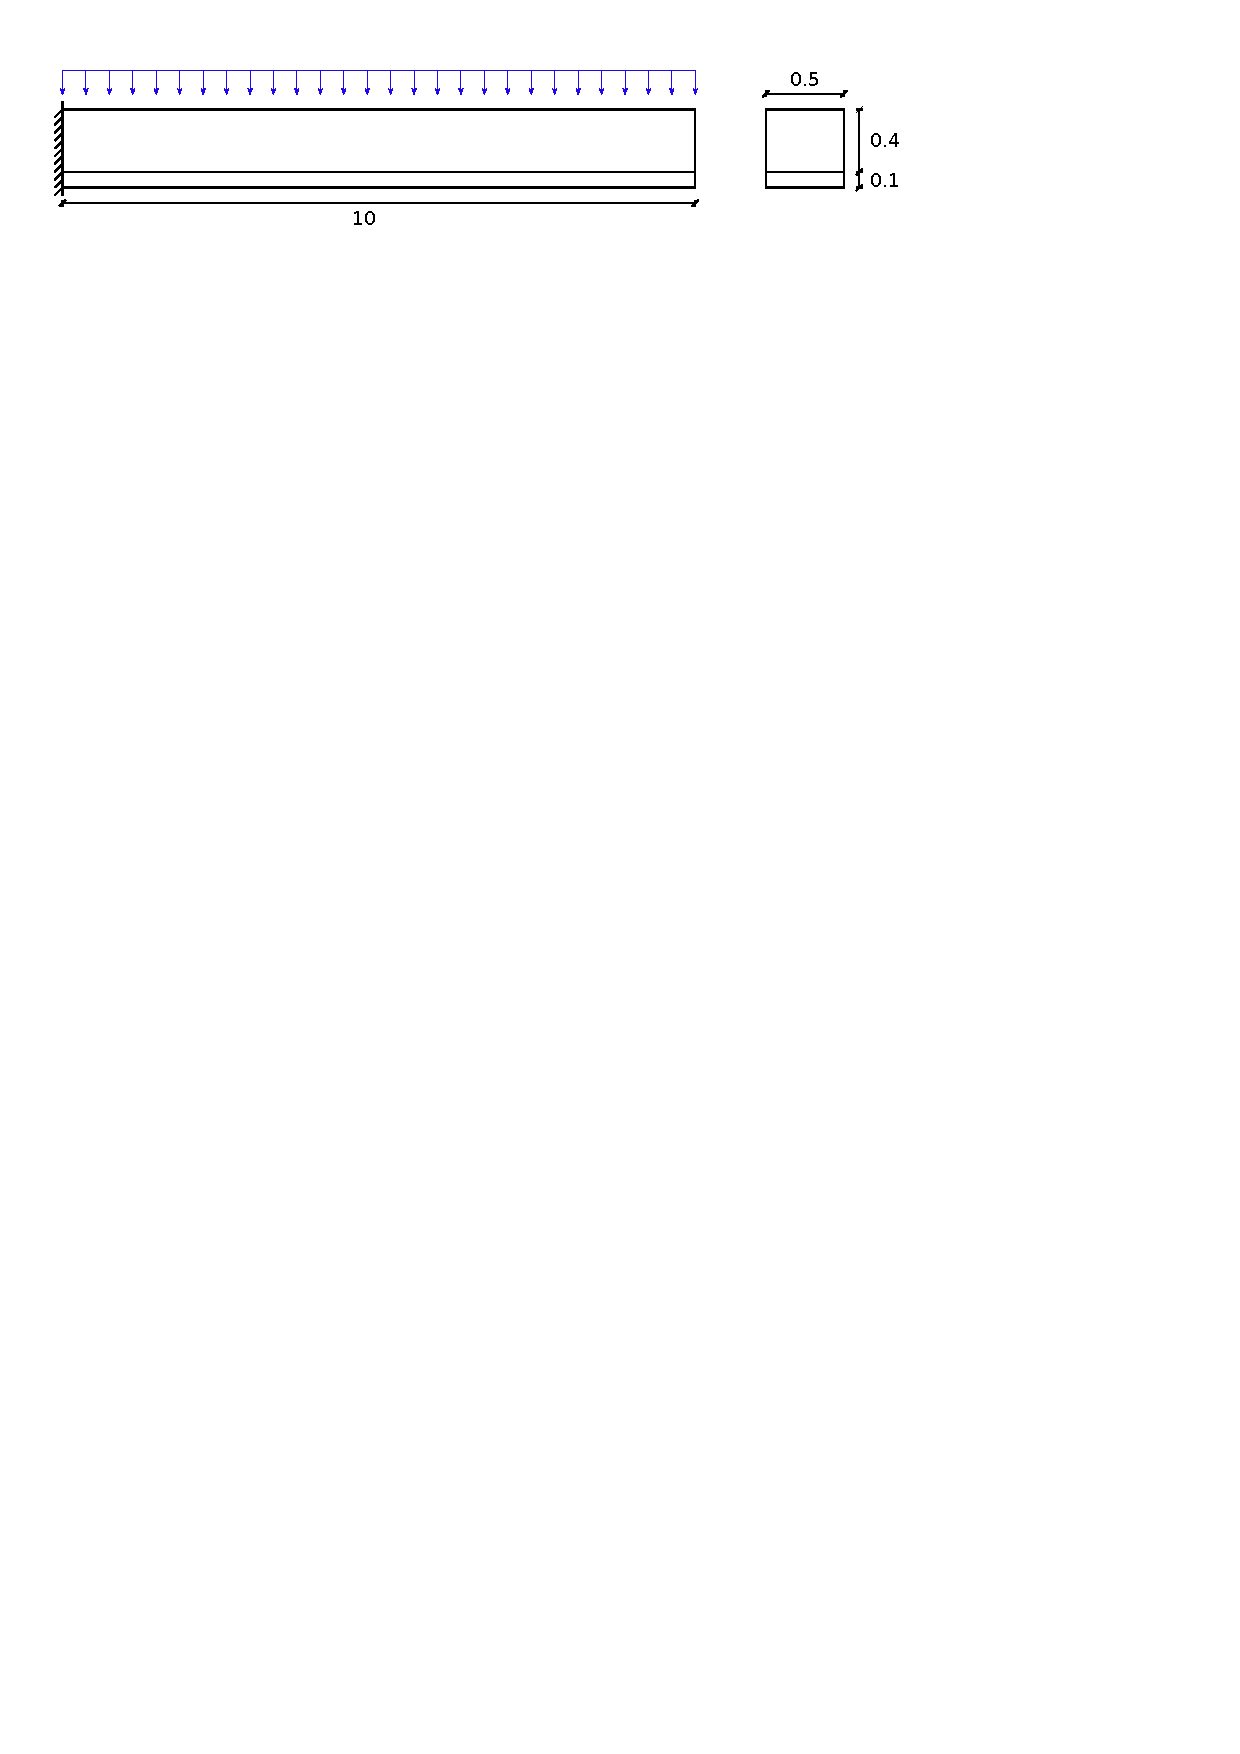
\includegraphics[width=0.9\textwidth]{Ejercicio4_2023-1.pdf}
\end{center}
\end{document}
